%%%%%%%%%%%%%%%%%%%%%%%%%%%%% Define Article %%%%%%%%%%%%%%%%%%%%%%%%%%%%%%%%%%
\documentclass{article}
%%%%%%%%%%%%%%%%%%%%%%%%%%%%%%%%%%%%%%%%%%%%%%%%%%%%%%%%%%%%%%%%%%%%%%%%%%%%%%%

%%%%%%%%%%%%%%%%%%%%%%%%%%%%% Using Packages %%%%%%%%%%%%%%%%%%%%%%%%%%%%%%%%%%
\usepackage{cmap}
\usepackage{geometry}
\usepackage{graphicx}
\usepackage{amssymb}
\usepackage{amsmath}
\usepackage{amsthm}
\usepackage{empheq}
\usepackage{mdframed}
\usepackage{booktabs}
\usepackage{lipsum}
\usepackage{graphicx}
\graphicspath{ {./images/} }
\usepackage{color}
\usepackage{psfrag}
\usepackage[fleqn]{nccmath}
\usepackage{comment}
\usepackage{pgfplots}
\usepackage{sidecap}
\usepackage{bm}
\usepackage{physics}
\usepackage{wrapfig}
\usepackage{listings}
\def\magyarOptions{suggestions=no} % nem tudom miért de kell ez a sor
\usepackage[magyar]{babel}
%%%%%%%%%%%%%%%%%%%%%%%%%%%%%%%%%%%%%%%%%%%%%%%%%%%%%%%%%%%%%%%%%%%%%%%%%%%%%%%

%%%%%%%%%%%%%%%%%%%%%%%%%% Page Setting %%%%%%%%%%%%%%%%%%%%%%%%%%%%%%%%%%%%%%%
\geometry{a4paper}


%%%%%%%%%%%%%%%%%%%%%%%%%% Define some useful colors %%%%%%%%%%%%%%%%%%%%%%%%%%
\definecolor{ocre}{RGB}{243,102,25}
\definecolor{mygray}{RGB}{243,243,244}
\definecolor{deepGreen}{RGB}{26,111,0}
\definecolor{shallowGreen}{RGB}{235,255,255}
\definecolor{deepBlue}{RGB}{61,124,222}
\definecolor{shallowBlue}{RGB}{235,249,255}
%%%%%%%%%%%%%%%%%%%%%%%%%%%%%%%%%%%%%%%%%%%%%%%%%%%%%%%%%%%%%%%%%%%%%%%%%%%%%%%

%%%%%%%%%%%%%%%%%%%%%%%%%% Define an orangebox command %%%%%%%%%%%%%%%%%%%%%%%%
\newcommand{\orangebox}[1]{\fcolorbox{ocre}{mygray}{\hspace{1em}#1\hspace{1em}}}
%%%%%%%%%%%%%%%%%%%%%%%%%%%%%%%%%%%%%%%%%%%%%%%%%%%%%%%%%%%%%%%%%%%%%%%%%%%%%%%

%%%%%%%%%%%%%%%%%%%%%%%%%%%% English Environments %%%%%%%%%%%%%%%%%%%%%%%%%%%%%
\newtheoremstyle{mytheoremstyle}{3pt}{3pt}{\normalfont}{0cm}{\rmfamily\bfseries}{}{1em}{{\color{black}\thmname{#1}~\thmnumber{#2}}\thmnote{\,--\,#3}}
\newtheoremstyle{myproblemstyle}{3pt}{3pt}{\normalfont}{0cm}{\rmfamily\bfseries}{}{1em}{{\color{black}\thmname{#1}~\thmnumber{#2}}\thmnote{\,--\,#3}}
\theoremstyle{mytheoremstyle}
\newmdtheoremenv[linewidth=1pt,backgroundcolor=shallowGreen,linecolor=deepGreen,leftmargin=0pt,innerleftmargin=20pt,innerrightmargin=20pt,]{theorem}{Theorem}[subsection]
\theoremstyle{mytheoremstyle}
\newmdtheoremenv[linewidth=1pt,backgroundcolor=shallowBlue,linecolor=deepBlue,leftmargin=0pt,innerleftmargin=20pt,innerrightmargin=20pt,]{definition}{Definition}[subsection]
\theoremstyle{myproblemstyle}
\newmdtheoremenv[linecolor=black,leftmargin=0pt,innerleftmargin=10pt,innerrightmargin=10pt,]{problem}{Problem}[subsection]
%%%%%%%%%%%%%%%%%%%%%%%%%%%%%%%%%%%%%%%%%%%%%%%%%%%%%%%%%%%%%%%%%%%%%%%%%%%%%%%

%%%%%%%%%%%%%%%%%%%%%%%%%%%%%%% Plotting Settings %%%%%%%%%%%%%%%%%%%%%%%%%%%%%
\usepgfplotslibrary{colorbrewer}
\pgfplotsset{width=8cm, compat=1.9}
%%%%%%%%%%%%%%%%%%%%%%%%%%%%%%%%%%%%%%%%%%%%%%%%%%%%%%%%%%%%%%%%%%%%%%%%%%%%%%%

%%%%%%%%%%%%%%%%%%%%%%%%%%%%%%% Title & Author %%%%%%%%%%%%%%%%%%%%%%%%%%%%%%%%
\title{Cím}
\author{Princzes
Barnabás}
%%%%%%%%%%%%%%%%%%%%%%%%%%%%%%%%%%%%%%%%%%%%%%%%%%%%%%%%%%%%%%%%%%%%%%%%%%%%%%%


\begin{document}
\selectlanguage{magyar}
\maketitle
\begin{abstract}
    Lent hagytam a füzetem és jövő héten doga szóval time to kick ass!
    Írjunk egy jó kis jegyzetet.
\end{abstract}
\section{Előadás}
\subsection{Alapok}
Van a \{$B$\}$A$\{$K$\} azaz a Bemeneti
feltétel (egy logikai állítás) Algoritmus és Kimeneti feltétel
(szintén egy logikai állítás).
\\
Legyen $A$ algoritmus. $e_1,\ldots,e_m$ elemi műveletek az algoritmusban
és $t_i$ az edott $e_i$-hez tartozó időigény. Az algoritmus tényleges futási ideje
$T(A,x)$ ahol x egy bemenet és a bemenet mérete $|x|$ például
(tömb, halmaz\ldots) esetében az elemek száma.
Az $e_i$ és $t_i$ és $|x|$ együtt a bonyolultság mértéke.

\subsection{Esetek}
\begin{itemize}
    \item Legjobb eset: \[T_{lj} = \min \{T(A,x):|x|=n\}\]
    \item Legrosszabb eset: \[T_{lr} = \max\{T(A,x):|x|=n\}\]
    \item Átlagos eset: Legyen $\Pr(x)$ annak
          a valószínűsége, hogy épp $x$ lesz
          $A$ algoritmus bemenete, ekkor:
          \\ \[T_a(A,n) = \sum_{|x|=n}\Pr(x)T(A,x)\]
\end{itemize}
\begin{center}
    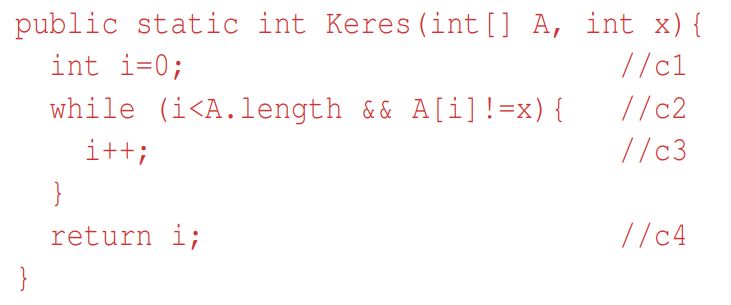
\includegraphics[height=4cm]{keres}
    \\
    Itt Keres$(A,n,x)$ futási ideje: $c_1+(i+1)c_2+ic_3+c_4$
\end{center}

$$T_{lj} = c_1+c_2+c_4 = O(1)$$
$$T_{lr} = c_1+(n+1)c_2+nc_3+c_4=(c_2+c_3)n+c_1+c_2+c_4=O(n)$$
Az átlagos eset számításához vezessünk be pár fogalmat:\\
Legyen $B_0$ a legjobb bemeneti eset amikor is egyből megtaláljuk a keresett elemet\\
Legyen $B_n$ amikor nem találjuk meg.\\
Minden lehetséges bemenet $\in B_i\ |\ i=0,\ldots,n-1$ \\
Legyen $D$ az Integer összes lehetséges értéke (nagy szám).\\
Annak hogy az keresendő számot pont kiszúrjuk a valószínűsége: $p=\frac{1}{D}$\\
Annak, hogy egy olyat találunk amelyik nem a keresett szám: $q=1-\frac{1}{D}$\\
$Pr((A,n,x)\in B_i) = q^ip, i=0,\ldots,n-1$\\
Itt $q^i$ jelöli, hogy hányszor nem találtuk meg és $p$ amikor megtaláltuk.
Az utolsó lehetséges esetnél viszont csak $q$ eset fordul elő az pedig $n$-szer
ugyanis végigmegyünk és nem találjuk meg a keresett elemet.
$Pr((A,n,x)\in B_n) = q^n, $\\

$$T_a(n) = \sum_{i=0}^n  Pr((A,n,x)\in B_i)(c1 + (i+1)c2 +ic3 +c4)$$
Az átlagos esetet úgy kapjuk meg, ha minden lehetséges bemenet futási idejét
megszorozzuk az adott bemenet valószínűségével és az eseteket összeadjuk.\\
A $B_n$ bemenetre vonatkozó eset specifikus így emeljük ki a többi közül:
$$T_a(n) = q^n(c1 + (n+1)c2 +nc3 +c4)+\sum_{i=0}^{n-1} q^ip(c1 + (i+1)c2 +ic3 +c4)$$
Mivel $q^n\to0$ (0-hoz tart) ezért felfele kerekítjük 1-re.
Mivel a $\Sigma$ alatt mindent beszorzunk
$p(\ldots)$-al ahol a zárojelben $i<n$ így azt ki is emelhetjük ugyanúgy felfele
kerekítve $i$-t és $i+1$-et kicserélve $n$-re.
$$T_a(n)\lessapprox\hat{T_a(n)}=(c1+(i+1)c2+ic3+c4)+(c_1+n(c_2+c_3)+c_4)p\sum_{i=0}^{n-1}q^i$$
A $\Sigma$ tag egyenlő a mértani sorozat összegképletével, behelyettesítjük:
$$\hat{T_a(n)}=(c1+(i+1)c2+ic3+c4)+(c_1+n(c_2+c_3)+c_4)p\frac{q^n-1}{q-1}$$
Mivel $p=1-q$ ezért átalakítunk:
$$\hat{T_a(n)}=(c1+(i+1)c2+ic3+c4)+(c_1+n(c_2+c_3)+c_4)(1-q^n)$$
Mivel $(1-q^n)\to1$ megint felfele kerekítünk, majd összevonunk.
$$\hat{T_a(n)}\lessapprox\hat{\hat{T_a(n)}}=(2c_2+2c_3)n+2c_1+c_2+2c_4$$
Itt pedig $n$ a domináns tag szóval:
$$T_a(n)=O(n)$$


\subsection{Praktikus képletek}
\begin{align*}
    T_{lj}=            & \min \{T(A,x):|x|=n\}                                                                 \\
    T_{lr}=            & \max\{T(A,x):|x|=n\}                                                                  \\
    T_a(A,n)=          & \sum_{|x|=n}\Pr(x)T(A,x)                                                              \\
    \sum_{i=1}^{n}i=   & \frac{n(n+1)}{2}\quad(\text{$a_1=1$, $d=1$ speciális számtani sorozat összegképlete}) \\
    \sum_{i=1}^{n}i^2= & \frac{n(n+1)(2n+1)}{6}                                                                \\
    \sum_{i=1}^{n}n=   & n^2                                                                                   \\
    \sum_{i=m}^{n}q^i= & \frac{q^m-q^{n+1}}{1-q}\quad(\text{mértani sorozat összegképlete})
\end{align*}

\section{Függvények növekedési rendje}
\subsection{$O$ - Nagy ordó}
\[O(g(n))=\{f(n):(\exists c>0, n_0 \geq 0)(\forall n \geq n_0)
    \underline{(0 \leq f(n) \leq c g(n))}\}\]
Nagy ordó egy halmaz amelyekben adott függvények vannak, jelöljünk
egy ilyen függvényt  $f(n)$-el.
Ezek minden olyan $f(n)$ függvény ahol létezik egy $c$ konstans úgy,
 hogy lesz egy $n_0$
küszöbszám amire igaz, hogy minden $n_0$-nál nagyobb $n$-számra $f(n)$ nem negatív
és $cg(n)$ alatt van.\\
$f(n)\in O(g(n))$ helyett szoktuk a $f(n)=O(g(n))$ jelölést alkalmazni.

\begin{center}
    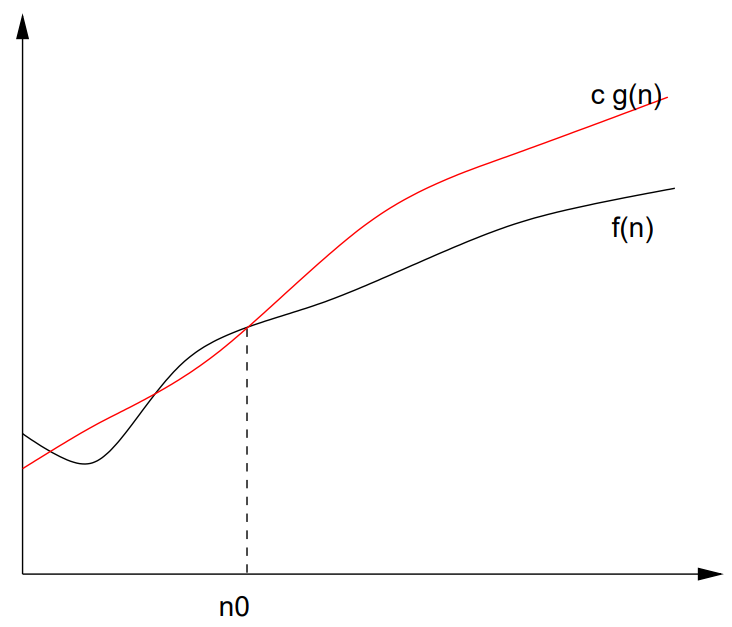
\includegraphics[height=6cm]{o}
    \\
    $f(n)=O(g(n))$ mivel $g(n)$-re tudunk választani olyan pozitív konstansot,
    hogy mindig $f(n)$ fölött maradjon.
\end{center}

\begin{center}
    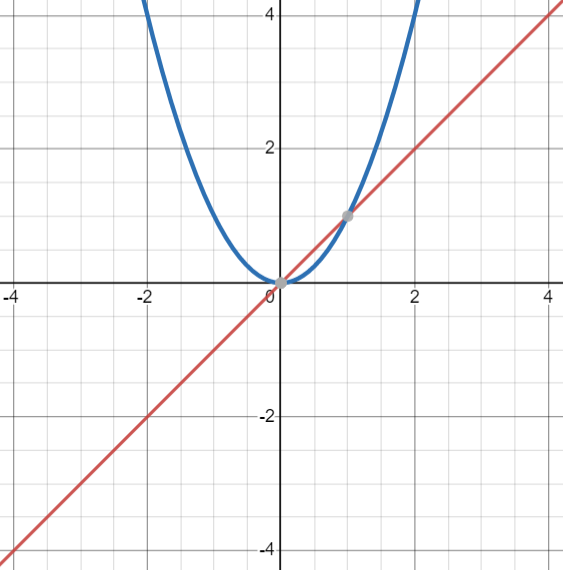
\includegraphics[height=6cm]{o2}\\
    Hasonlítsuk össze \color{red}$x$\color{black}\,és\,
    \color{blue}$x^2$\color{black}\,függvényt\\
    Nem tudunk olyan $c$ konstanst választani, hogy azzal
    $c$\,\color{red}$x$\color{black}\,egy
    $n_0$ érték fölött mindig nagyobb legyen mint
    \color{blue}$x^2$\color{black}\,ezért:\\
    $O($\color{red}$x$\color{black}$)\neq O($\color{blue}$x^2$\color{black}$)$
\end{center}

\subsection{$\Omega$ - Omega}
Ugyanaz mint a $O$ csak ez alulról korlátoz.
\[\Omega(g(n))=\{f(n):(\exists c>0,n_0\geq 0)(\forall n\geq n_0)
    \underline{(0\leq cg(n)\leq f(n))}
    \}\]

\subsection{$\Theta$ - Theta}
Ez alulról és felülről is korlátol. Azaz egy adott értéktől
a legjobb és a legrosszabb eset is ugyanazt a nagyságrendet követi.
\[\Theta(g(n))=\{f(n):(\exists c_1,c_2>0,n_0\geq 0)(\forall n\geq n_0)
    \underline{(0\leq c_1g(n)\leq f(n)\leq c_2g(n))}
    \}\]

\begin{comment}
\subsection{Nevezetes függvényosztályok}

\begin{center}
    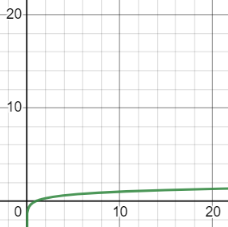
\includegraphics[height=3cm]{logx}\\Logaritmikus - $O(lg(n))$\\
    \newpage
    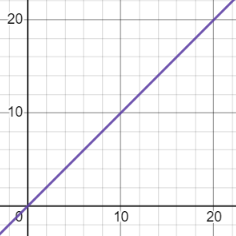
\includegraphics[height=3cm]{x}\\Lineáris - $O(n)$\\
    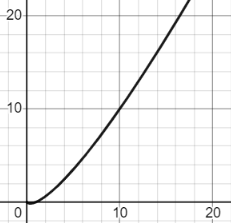
\includegraphics[height=3cm]{xlogx}\\$n log(n)$ - $O (nlg (n) )$\\
    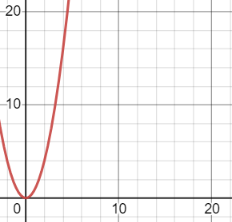
\includegraphics[height=3cm]{xx}\\Négyzetes - $O (n^2) $\\
    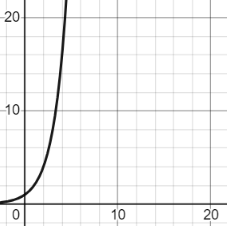
\includegraphics[height=3cm]{2onx}\\Exponenciális - $O (2^x)$\\
    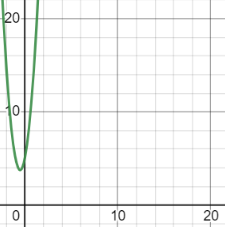
\includegraphics[height=3cm]{xpoli}\\\[\text{Polinomiális - }
    O(\sum_{i=0}^{k}a_i n^i)(a_k>0)\]\\
    Ez utóbbi a legösszetettebb így itt sokkal elővigyázatosabbnak kell lenni mikor
    azt nézzük, hogy melyiknél nagyobb.
\end{center}
\end{comment}

\section{Alkalmazás}
A fenti definíciók következményei:
\begin{itemize}
    \item 
    Ha $f(n) = O(g(n))$ azaz $f(n)$-t felülről határolja $g(n)$ akkor:
    \[0\leq \lim_{n\to\infty}\frac{f(n)}{g(n)}<\infty\]
    \item 
    Ha $f(n) = \Omega(g(n))$ azaz $f(n)$-t alulról határolja $g(n)$ akkor:
    \[0<\lim_{n\to\infty}\frac{f(n)}{g(n)}\leq \infty\]
    \item 
    Ha $f(n) = \Theta(g(n))$ azaz $f(n)$-t alulról és felülről is határolja $g(n)$, 
    azaz növekedési rendjük egyenesen arányos, akkor:
    \[0<\lim_{n\to\infty}\frac{f(n)}{g(n)}<\infty\]
\end{itemize}

\subsection{Praktikus képletek}
\begin{align*}
    n!\approx & \sqrt{2\pi n} { \left( \frac{n}{e} \right) }^n\\
\end{align*}


\end{document}
